% !TeX spellcheck = en_GB
\chapter{Supplemental figures}


\begin{figure}[ht]
	\centering
	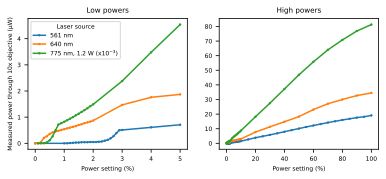
\includegraphics{laser_power}
	\caption{
		The power of each of the three lasers as measured through a 10x objective. Notice the non-linearity at low power settings. The 775 nm data was scaled down by three orders of magnitude.
	}
	\label{fig:laser power}
\end{figure}

\begin{figure}
	\centering
	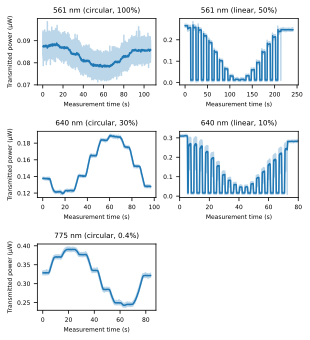
\includegraphics{laser_polarisation}
	\caption{
		Polarisation characterisation of the different lasers. To characterise circular polarisation, a polariser was placed in the sample and scanned from \ang{0} to \ang{180} in steps of \ang{20} (notice that I forgot to sample \ang{260} in the 775 nm data). Linear polarisation was characterised by fixing the polariser in place at \ang{0} and scanning the laser itself from \ang{0} to \ang{180} in steps of \ang{10}. Dark blue: average over 200 samples, light blue: raw data. 
	}
	\label{fig:laser polarisation}
\end{figure}
%\begin{figure}[ht]
%	\centering
%	\includegraphics{640 laser pol characteristics in sample}
%	\caption{
%		Polarisation characteristics at the sample plane of the 640 laser. \textbf{Left:} power transmitted through a stationary polariser aligned to maximise transmission of the 640 laser set to an polarisation of 0° (vertical in the sample plane), while the laser beam rotates. \textbf{Right:} power transmitted through a manually rotating polariser, while the beam is set to circular polarisation.
%	}
%	\label{fig:640 laser pol at sample}
%\end{figure}
%
%\begin{figure}[ht]
%	\centering
%	\includegraphics{561 laser pol characteristics in sample}
%	\caption{
%		Polarisation characteristics at the sample plane of the 561 laser. Left and right panes are the same as \autoref{fig:640 laser pol at sample}. (As the data on the left was acquired at 50\% laser power to increase the signal at minimum transmission, but the data on the right was acquired at 10\% laser power for safety reasons, the data on the right has been multiplied by a factor of 5 to allow comparison between the two figures. This also increased the noise.)
%	}
%	\label{fig:561 laser pol at sample}
%\end{figure}
%
%\begin{figure}[ht]
%	\centering
%	\includegraphics{775 laser pol characteristics in sample (donut beam, no psted optics)}
%	\caption{
%		Polarisation characteristics at the sample plane of the depletion beam, without pSTED optics. As its polarisation state cannot be manipulated through the software, only circular polarisation is characterised by manually rotating a polariser at the sample plane and measuring the transmitted power.
%	}
%	\label{fig:775 laser pol at sample}
%\end{figure}

\begin{figure}
	\centering
	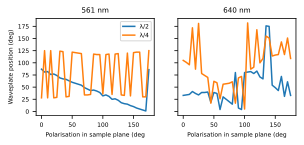
\includegraphics{excitation_waveplate_calibrations.pdf}
	\caption{
		Calibrations of the excitation waveplates, as supplied by the microscope manufacturer.
	}
	\label{fig:excitation waveplate calibration}
\end{figure}

\begin{figure}
	\centering
	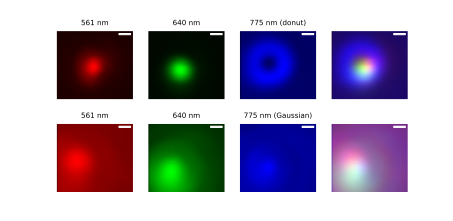
\includegraphics{laser_psfs.pdf}
	\caption{
		Point spread functions of the different lasers (in donut and Gaussian modes) at different SLM configurations, by measuring the reflection from 100 nm wide gold beads. Scale bars 200 nm.
	}
	\label{fig:normal psfs}
\end{figure}

\begin{figure}
	\centering
	\includegraphics{apd_pol_sensitivity.pdf}
	\caption{Dependence of the signal from APD1 on the angle of polarisation of incoming light.}
	\label{fig:apd pol sensitivity}
\end{figure}

\begin{figure}
\centering
\includegraphics{pol_cube.pdf}
\caption{Performance of the polarising beam splitter}
\label{fig:pol cube}
\end{figure}

\begin{figure}
	\centering
	\includegraphics{ssted_1.ai}
	\caption{
		Confocal (left) and STED (right) acquisitions of various fields of view.
	}
	\label{fig:ssted supplementary}
\end{figure}


\begin{figure}
	\centering
	\includegraphics{psted_hwp_offset.pdf}
	\caption{
		The rotating HWP I put in the beamline controls the depletion beam polarisation. With an offset of 38.5°, the depletion beam is parallel to the 640 laser (set to vertical linear polarisation).
	}
	\label{fig:psted hwp offset}
\end{figure}

\begin{figure}
	\centering
	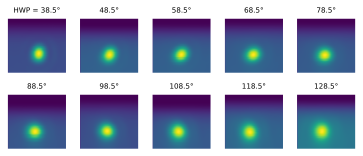
\includegraphics{psted_psfs.pdf}
	\caption{
		Depletion PSF as a function of beam polarisation. The figure titles indicate the angle of the HWP. The shown images are recentered on the pixel with the highest intensity to correct for displacement. Scale bars 100~nm.
	}
	\label{fig:psted psfs}
\end{figure}

\begin{figure}
	\centering
	\includegraphics{psted_psfs_orientation_and_power.pdf}
	\caption{
		\textbf{Left:} The pSTED PSF is elliptical, and its orientation matches the light polarisation. \textbf{Right:} pSTED intensity depends on polarisation. Error bars show standard deviation, n=10.
	}
	\label{fig:psted psf orientation and power}
\end{figure}

\begin{figure}
	\centering
	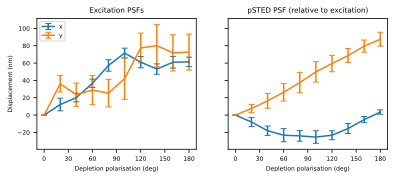
\includegraphics{psted_psfs_displacement.pdf}
	\caption{
		The displacement of the laser PSFs as a function of depletion polarisation. \textbf{Left:} The displacement of the 561~nm and 640~nm PSFs (representing drift in the image). \textbf{Right:} Displacement of the pSTED PSF relative to the excitation PSFs.
	}
\end{figure}